\clearpage

\section{Classical Y Stiffness: Microscopic
Derivation}\label{sec-nbcp-stiffness-appendix}

\subsection{Classical stiffness of the zero-SOC Y
state}\label{sec-nbcp-y-stiffness}

A microscopic baseline can be obtained at \(J_{\rm PD}=J_\Gamma=0\),
fixed longitudinal field and \(T=0\). The calculation below concerns the
locally stable classical Y branch, with \(J_z>J>0\), \(0<h<3SJ\) and a
positive Hessian on the remaining uniform modes. It gives the classical
coefficient \(\rho_s^{\rm cl}\), without its zero-point or thermal
renormalization. The endpoint with additional soft modes must be treated
separately.

\textbf{Bond energy and canting relaxation.}

Let \(c=\cos t\), \(s=\sin t=\sqrt{1-c^2}\) and choose the reference
vectors \(\mathbf n_A=(s,0,c)\), \(\mathbf n_B=(-s,0,c)\) and
\(\mathbf n_C=(0,0,-1)\). A physical twist is imposed at the actual site
position \(\mathbf r\):

\begin{equation}\phantomsection\label{eq-nbcp-y-spatial-twist}{
\mathbf S_\alpha(\mathbf r)
=S R_z(\mathbf Q\cdot\mathbf r)\mathbf n_\alpha,
\qquad
c=\frac{h+3SJ_z}{3S(J+J_z)}.
}\end{equation}

The vector \(\mathbf Q\) has units of inverse length; the angle
difference on a bond is \(\mathbf Q\cdot\boldsymbol\delta\). It is not a
common angle assigned to every site in a magnetic cell. Equivalently,
periodic boundaries carry the corresponding twist. The derivative at
\(\mathbf Q=0\) is taken on the branch continuously connected to this Y
state, rather than minimizing over different winding sectors.

Choose the oriented bond triplet \(\boldsymbol\delta_d=a(1,0)\),
\(a(-1/2,\sqrt3/2)\) and \(a(-1/2,-\sqrt3/2)\) for each cyclic
sublattice pair. There are nine bonds per three-spin cell, each physical
bond counted once. The triplet satisfies \(\sum_d\boldsymbol\delta_d=0\)
and \(\sum_d\delta_{d\mu}\delta_{d\nu}=3a^2\delta_{\mu\nu}/2\). At fixed
internal vectors, only the A-B bonds contribute transverse exchange.
Defining

\begin{equation}\phantomsection\label{eq-nbcp-y-twist-structure-factor}{
\gamma(\mathbf Q)=\frac13\sum_{d=1}^3
\cos(\mathbf Q\cdot\boldsymbol\delta_d)
=1-\frac{a^2|\mathbf Q|^2}{4}
+O(a^4|\mathbf Q|^4),
}\end{equation}

the energy per physical spin is

\begin{equation}\phantomsection\label{eq-nbcp-y-twisted-energy}{
e_Y(\mathbf Q,c)=S^2\left[
-J(1-c^2)\gamma(\mathbf Q)+J_z(c^2-2c)\right]
-\frac{hS}{3}(2c-1).
}\end{equation}

The three A-B bonds contribute \(S^2[-J(1-c^2)\gamma+J_zc^2]\) per spin;
the three B-C and three C-A bonds each contribute \(-J_zS^2c\). The
division by three physical spins has already been made in each
contribution. The field term follows from
\(S(n_A^z+n_B^z+n_C^z)=S(2c-1)\) per cell. Consequently,

\begin{equation}\phantomsection\label{eq-nbcp-y-canting-relaxation}{
\begin{aligned}
\partial_c e_Y&=2S^2\{[J\gamma(\mathbf Q)+J_z]c-J_z\}
-\frac{2hS}{3},\\
c_*(\mathbf Q)&=\frac{J_z+h/(3S)}{J_z+J\gamma(\mathbf Q)}
=c_0+\frac{c_0Ja^2|\mathbf Q|^2}{4(J+J_z)}+O(|\mathbf Q|^4),
\end{aligned}
}\end{equation}

where \(c_0\) is the untwisted value in
Eq.~\ref{eq-nbcp-y-spatial-twist}, denoted by \(c\) below. Since
\(\partial_c e_Y(0,c_0)=0\) and \(c_*-c_0=O(Q^2)\), this canting
relaxation changes the energy only at \(O(Q^4)\). At quadratic order the
explicit \(\gamma\) dependence therefore gives

\begin{equation}\phantomsection\label{eq-nbcp-y-twist-cost}{
e_Y(\mathbf Q)-e_Y(0)
=\frac{JS^2(1-c^2)a^2}{4}|\mathbf Q|^2
+O(|\mathbf Q|^4).
}\end{equation}

\textbf{Regular coordinates and the full internal Hessian.}

Varying \(t\) alone does not test all possible internal relaxations.
Introduce orthonormal tangent vectors

\begin{equation}\phantomsection\label{eq-nbcp-y-regular-tangents}{
\begin{aligned}
\mathbf e_{\theta A}&=(c,0,-s),&
\mathbf e_{\theta B}&=(c,0,s),&
\mathbf e_{\theta C}&=(-1,0,0),\\
\mathbf e_{\varphi\alpha}&=(0,1,0),&
\mathbf n_\alpha(\boldsymbol\xi)&=
\mathbf n_\alpha\sqrt{1-x_\alpha^2-y_\alpha^2}
+\mathbf e_{\theta\alpha}x_\alpha+\mathbf e_{\varphi\alpha}y_\alpha.
\end{aligned}
}\end{equation}

The variables \(\boldsymbol\xi=(x_A,x_B,x_C,y_A,y_B,y_C)^{\mathsf T}\)
are dimensionless transverse components. In particular, \(y_C\) is a
regular Cartesian component, not the singular azimuth of the axial C
spin. Expanding a single bond gives a cross term
\(S^2\mathbf e_{u i}^{\mathsf T}\mathsf J\mathbf e_{v j}\xi_{u i}\xi_{v j}\)
and a length-constraint term
\(-S^2(\mathbf n_i^{\mathsf T}\mathsf J\mathbf n_j)(x_i^2+y_i^2+x_j^2+y_j^2)/2\).
The field adds \(hS n_i^z(x_i^2+y_i^2)/2\). Summing all nine bonds and
using stationarity gives the cell Hessian

\begin{equation}\phantomsection\label{eq-nbcp-y-uniform-hessian}{
\begin{gathered}
\mathcal K_0=\begin{pmatrix}K_x&0\\0&K_y\end{pmatrix},\qquad
U=-J_z+c^2(J+J_z),\quad Z=J_z+c(J_z-J),\\
K_x=3S^2\begin{pmatrix}J&U&-cJ\\U&J&-cJ\\-cJ&-cJ&Z\end{pmatrix},\qquad
K_y=3S^2\begin{pmatrix}J&J&J\\J&J&J\\J&J&Z\end{pmatrix}.
\end{gathered}
}\end{equation}

A common physical rotation has tangent
\(\mathbf g=(0,0,0,s,-s,0)^{\mathsf T}\), so
\(\boldsymbol\xi=\mathbf g\phi+O(\phi^2)\) and
\(\mathcal K_0\mathbf g=0\). The norm of \(\mathbf g\) is not set to
one: \(\phi\) retains its meaning as an angle in radians. If
\(\mathbf e_{x_A},\ldots,\mathbf e_{y_C}\) denote the six coordinate
unit vectors, choose the five-column projector

\begin{equation}\phantomsection\label{eq-nbcp-y-hard-projector}{
\mathsf P=\left(\mathbf e_{x_A},\mathbf e_{x_B},\mathbf e_{x_C},
\frac{\mathbf e_{y_A}+\mathbf e_{y_B}}{\sqrt2},\mathbf e_{y_C}\right),
\qquad H=\mathsf P^{\mathsf T}\mathcal K_0\mathsf P.
}\end{equation}

This removes only the uniform phase; both C-spin tilts remain. Local
stability requires \(H>0\). Let \(\mathbf z\) denote these five hard
coordinates. The cell energy has quadratic expansion

\begin{equation}\phantomsection\label{eq-nbcp-y-stiffness-relaxation}{
\delta E_{\rm cell}
=\frac12\mathbf z^{\mathsf T}\mathsf K\mathbf z
+\mathbf z^{\mathsf T}\mathsf L\mathbf Q
+\frac12\mathbf Q^{\mathsf T}\mathsf D\mathbf Q+\cdots,
\qquad
\mathsf D_{\rm relaxed}
=\mathsf D-\mathsf L^{\mathsf T}\mathsf K^{-1}\mathsf L.
}\end{equation}

Here \(\mathsf K=H\) is the positive Hessian on the hard subspace.
Completing the square gives \(\mathbf z_*=-H^{-1}\mathsf L\mathbf Q\)
and lowers the quadratic energy by
\(\mathbf Q^{\mathsf T}\mathsf L^{\mathsf T}H^{-1}\mathsf L\mathbf Q/2\).
Inverting the full singular \(\mathcal K_0\) would not define this
relaxation. In the present XXZ model, differentiating a bond rotation
once with respect to \(Q_\mu\) produces a factor \(\delta_{d\mu}\)
multiplying the same spin expression for all three orientations. The
vanishing first bond moment therefore gives \(\mathsf L=0\), including
the axial-spin directions. The relaxed displacement starts at
\(O(|\mathbf Q|^2)\), and its energy correction starts at
\(O(|\mathbf Q|^4)\). Thus Eq.~\ref{eq-nbcp-y-twist-cost} already gives
the relaxed quadratic coefficient. This argument relies on the
bond-independent XXZ exchange and must be rechecked when SOC is
introduced.

Matching \(\delta e=a_{\rm spin}\rho_s^{\rm cl}|\mathbf Q|^2/2\) with
\(a_{\rm spin}=\sqrt3a^2/2\) gives the isotropic tensor

\begin{equation}\phantomsection\label{eq-nbcp-y-classical-stiffness}{
\rho_{\mu\nu}^{\rm cl}=\rho_s^{\rm cl}\delta_{\mu\nu},
\qquad
\boxed{\rho_s^{\rm cl}
=\frac{JS^2}{\sqrt3}\left[
1-\left(\frac{h+3SJ_z}{3S(J+J_z)}\right)^2\right]}.
}\end{equation}

The stiffness has units of energy. The lattice spacing cancels because
both the bond second moment and the area per spin scale as \(a^2\); the
magnetic-cell area is three times the latter and cannot replace it
without also changing the energy normalization. The result approaches
zero on the Y side of the classical UUD boundary, where the transverse Y
component disappears.

\textbf{Longitudinal response and the energy slope.}

For completeness, the susceptibility can be obtained from the same
Hessian. The cell magnetization changes by
\(\delta M_z=\mathbf w^{\mathsf T}\mathbf x\), with
\(\mathbf w=-S(s,-s,0)^{\mathsf T}\). An additional longitudinal field
\(\delta h\) produces the energy
\(\mathbf x^{\mathsf T}K_x\mathbf x/2-\delta h\,\mathbf w^{\mathsf T}\mathbf x\).
Minimizing gives \(\mathbf x_*=K_x^{-1}\mathbf w\,\delta h\). Since

\begin{equation}\phantomsection\label{eq-nbcp-y-hessian-response}{
\begin{aligned}
K_x\mathbf w&=3S^2(J+J_z)s^2\mathbf w,\\
\chi_{\rm cell}&=\mathbf w^{\mathsf T}K_x^{-1}\mathbf w
=\frac{2S^2s^2}{3S^2(J+J_z)s^2}
=\frac{2}{3(J+J_z)},\qquad
\chi_z=\frac{\chi_{\rm cell}}{3},
\end{aligned}
}\end{equation}

\(\chi_z\) is the response per spin to the field energy \(h\), without
an additional \((g_z\mu_B)^2\) factor. It is also the coefficient of the
phase kinetic term after eliminating the conjugate hard mode at this
order. The division by three converts the magnetic-cell response to the
convention used in the continuum energy.

At zero SOC the pinning curvature vanishes. Combining the relaxed
susceptibility \(\chi_z=2/[9(J+J_z)]\) from
Eq.~\ref{eq-lswt-yv-pg-y-response} with
Eq.~\ref{eq-nbcp-phase-dispersion} predicts the leading energy slope

\begin{equation}\phantomsection\label{eq-nbcp-y-stiffness-dispersion}{
\varepsilon(\mathbf k)=u_Y|\mathbf k|+o(|\mathbf k|),
\qquad
u_Y^2=\frac{a_{\rm spin}\rho_s^{\rm cl}}{\chi_z}
=\frac94 a^2JS^2(J+J_z)(1-c^2).
}\end{equation}

The symbol \(u_Y\) is an energy times a length; the physical group
velocity is \(u_Y/\hbar\). At \(B=0.2\) T with the current comparison
parameters, \(c=0.804246889926\), \(\rho_s^{\rm cl}=0.00382336077954\)
meV and \(u_Y/a=0.0545895118739\) meV. No lattice spacing in metres has
been assumed.

The symbolic calculation verifies the stationarity equations, both bond
moments, the zero mixed Hessian, the Goldstone null vector, the
susceptibility and the formulas above. Numerical checks use five fields,
four Cartesian directions and four twist or momentum magnitudes
\(qa=0.03,0.01,0.003,0.001\). The static estimator is
\([e_*(\mathbf Q)+e_*(-\mathbf Q)-2e_*(0)]/(a_{\rm spin}|\mathbf Q|^2)\),
where all five internal variables are relaxed at each twist. The dynamic
estimator is
\(\chi_z[\varepsilon(\mathbf k)/|\mathbf k|]^2/a_{\rm spin}\), using the
lowest positive production-LSWT energy at nonzero \(\mathbf k\) without
a gap regulator.

\begin{longtable}[]{@{}rrr@{}}
\toprule\noalign{}
\(B\) (T) & \(\rho_s^{\rm cl}\) (meV) & \(u_Y/a\) (meV) \\
\midrule\noalign{}
\endfirsthead
\toprule\noalign{}
\(B\) (T) & \(\rho_s^{\rm cl}\) (meV) & \(u_Y/a\) (meV) \\
\midrule\noalign{}
\endhead
\bottomrule\noalign{}
\caption{Classical zero-SOC Y stiffness and phase velocity versus magnetic field.}\label{tab-nbcp-c-y-stiffness-1}\\
\endlastfoot
0.05 & 0.0059685633 & 0.0682058257 \\
0.10 & 0.0052969722 & 0.0642540367 \\
0.20 & 0.0038233608 & 0.0545895119 \\
0.30 & 0.0021758436 & 0.0411813340 \\
0.40 & 0.0003544207 & 0.0166205783 \\
\end{longtable}

At the smallest tested magnitude, the largest relative deviations over
these fields and directions are \(2.79\times10^{-6}\) for the
relaxed-energy estimator and \(2.56\times10^{-6}\) for the LSWT
estimator. These are convergence diagnostics, not bounds on physical
corrections. An independently assembled Cartesian constrained Hessian
reproduces the production-LSWT energies within \(1.10\times10^{-13}\)
meV. A separately enumerated 36-site triangular torus with twisted
boundaries reproduces the three-site energy within
\(2.09\times10^{-17}\) meV/spin for the sampled configurations. These
checks use the same XXZ model and parameters; they do not constitute an
independent experimental or many-body validation.

\begin{figure}

\centering{

\nbcpbounded{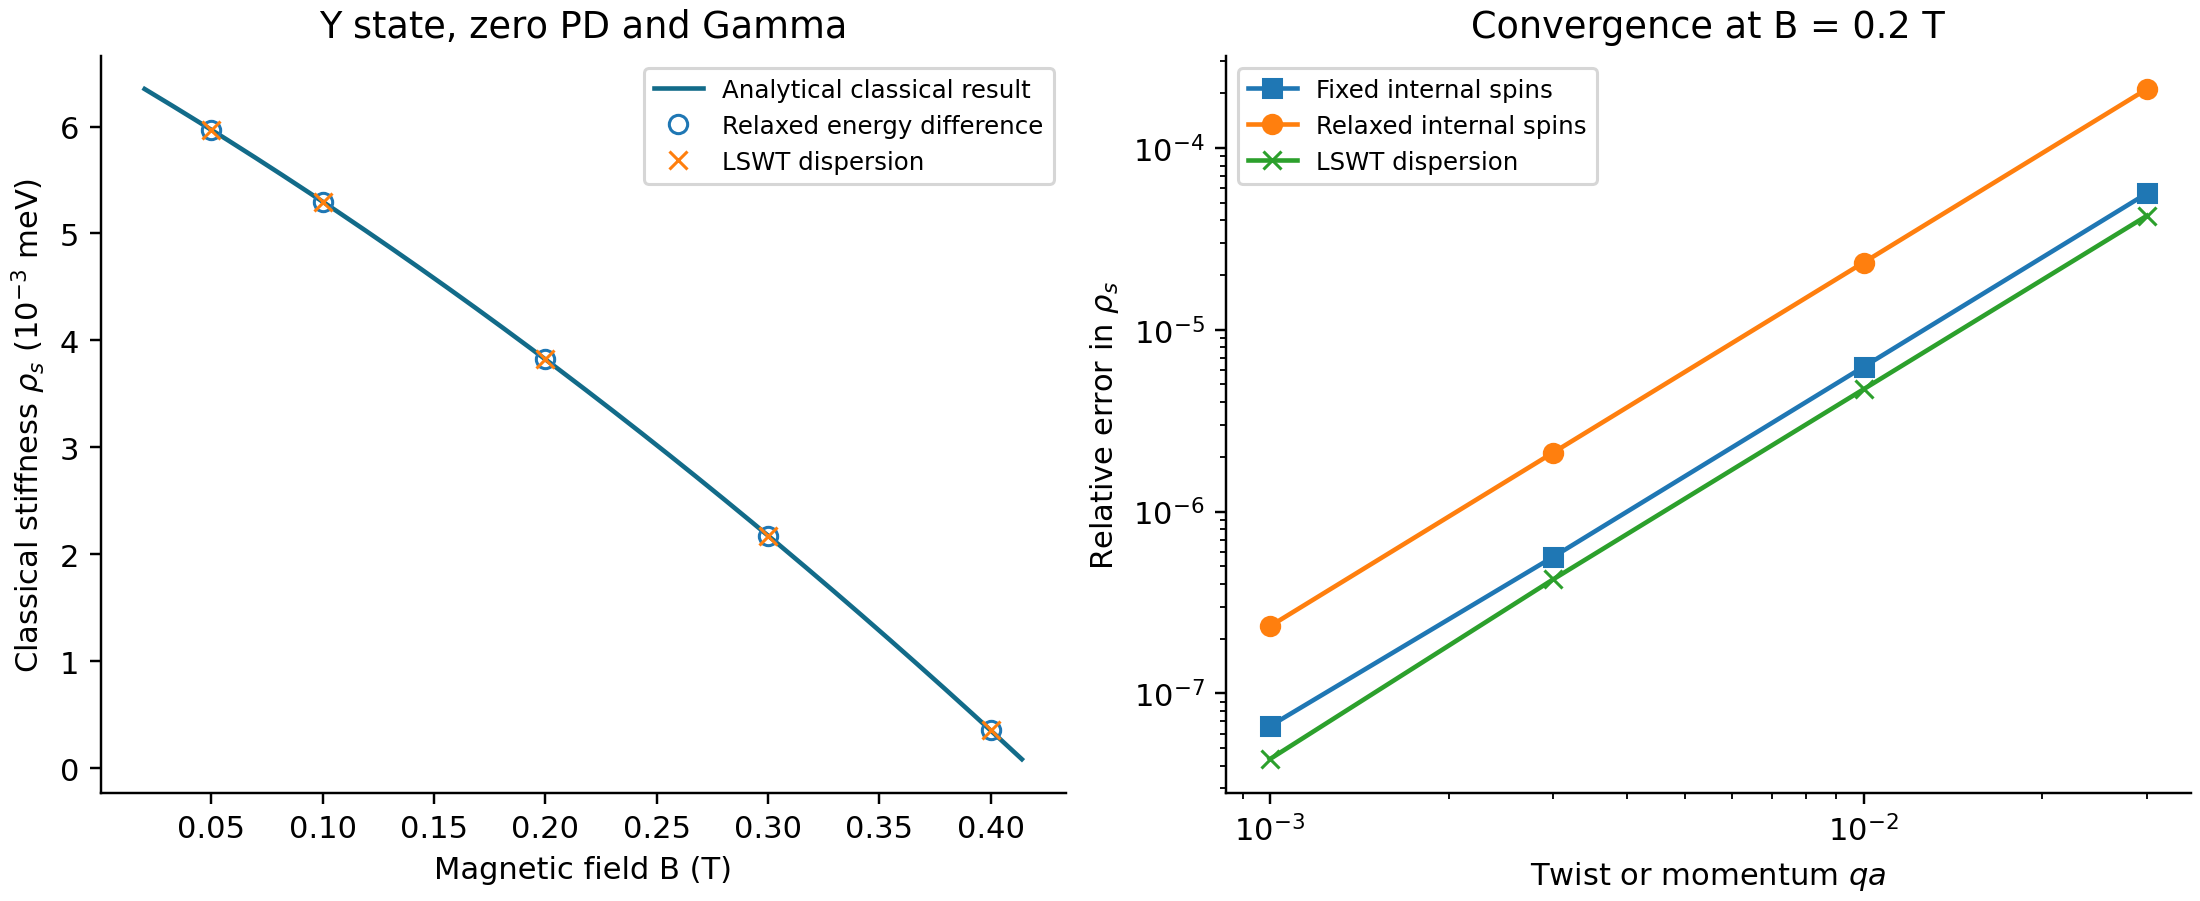
\includegraphics[keepaspectratio]{../../data-space/verification/260917-y-stiffness/y-stiffness-validation.png}}

}

\caption{\label{fig-nbcp-y-stiffness}Classical Y-state stiffness at zero
bond-dependent SOC. The energy-difference and LSWT estimates approach
the same analytical coefficient. The right panel shows convergence at
0.2 T along the Cartesian x direction; the numerical checks also include
three other directions.}

\end{figure}%

This baseline supplies a microscopic spatial coefficient for Y at zero
SOC. Its extension to classical Y with SOC is examined next. The
stiffness of V, the zero-point correction and the renormalized stiffness
entering the finite-temperature clock flow are not supplied by this
baseline. Positive local stiffness alone does not establish global phase
stability or a finite-temperature supersolid.

\subsection{Conditions for extending Y to
SOC}\label{sec-nbcp-y-soc-conditions}

The classical uniform Y family remains stationary when the
nearest-neighbor SOC tensors sum to zero over bond orientations. This
does not preserve global spin-\(z\) rotation as a symmetry of the
Hamiltonian. The distinction matters for a spatially varying phase: the
uniform energy and its Hessian can remain independent of the angle while
the gradient coefficients depend on that angle. The following
calculation is a classical harmonic expansion about a specified member
\(\phi_0\) of the Y family. It does not yet select \(\phi_0\) by the
quantum vacuum energy.

\textbf{Why the uniform-twist shortcut must be replaced.}

For two sites with angles \(\phi_i\) and
\(\phi_j=\phi_i+\mathbf Q\cdot(\mathbf r_j-\mathbf r_i)\), the bond
energy contains

\begin{equation}\phantomsection\label{eq-nbcp-y-soc-twist-obstruction}{
\mathbf n_i^{\mathsf T}R_z(\phi_i)^{\mathsf T}\mathsf J_d R_z(\phi_j)\mathbf n_j
=\mathbf n_i^{\mathsf T}
\bigl[R_z(\phi_i)^{\mathsf T}\mathsf J_d R_z(\phi_i)\bigr]
R_z\bigl(\mathbf Q\cdot(\mathbf r_j-\mathbf r_i)\bigr)\mathbf n_j.
}\end{equation}

In XXZ the bracket equals \(\mathsf J_d\). With SOC it depends on the
absolute phase \(\phi_i\). Replacing this bracket by a fixed tensor in a
three-site cell therefore does not describe a global spiral with SOC.
Instead, perturb a fixed background by a small-amplitude phase wave,
\(\phi(\mathbf r)=\phi_0+\epsilon\cos(\mathbf k\cdot\mathbf r)\), and
let all five internal coordinates relax. Take \(\epsilon\to0\) first,
then \(\mathbf k\to0\). This defines a local gradient coefficient
without sampling the whole angular orbit in space.

The momentum sign follows the toolkit bond convention. A stored
displacement is \(\mathbf d=\mathbf r_i-\mathbf r_j\), so the partner
sits at \(\mathbf r_j=\mathbf r_i-\mathbf d\) and the Fourier factor is
\(e^{-\mathrm i\mathbf k\cdot\mathbf d}\). The toolkit has compared this
construction element by element with the NBCP builders and has matched
its particle block to Bloch states rebuilt from exact one-magnon
eigenstates. The \(\mathbf k\) below is therefore the physical Bloch
momentum. Reversing every displacement would leave the even stiffness
unchanged and reverse the odd dispersion term. A laboratory direction
for that odd term additionally requires the orientation of the model
\(x\) axis, along \(\boldsymbol\delta_1\), relative to the crystal axes;
this is a material input that is not fixed here.

Write \(p=J_{\rm PD}\) and \(\Gamma=J_\Gamma\) in the following
formulas, with the exchange matrices defined in
Eq.~\ref{eq-nbcp-bond-matrix}. For stored
\(\mathbf d=a(\cos\varphi_d,\sin\varphi_d)\) and
\(\varphi_d=0,2\pi/3,4\pi/3\), the uniform sum is
\(\sum_d\mathsf J_d=3\operatorname{diag}(J,J,J_z)\), but its first
moments are

\begin{equation}\phantomsection\label{eq-nbcp-y-soc-first-moments}{
\begin{aligned}
M_x=\sum_d d_x\mathsf J_d
&=a\begin{pmatrix}3p&0&0\\0&-3p&3\Gamma/2\\0&3\Gamma/2&0\end{pmatrix},\\
M_y=\sum_d d_y\mathsf J_d
&=a\begin{pmatrix}0&-3p&-3\Gamma/2\\-3p&0&0\\-3\Gamma/2&0&0\end{pmatrix}.
\end{aligned}
}\end{equation}

Consequently, the zero first moment of the \emph{unweighted} bond
vectors no longer implies a vanishing phase-gradient coupling to the
hard coordinates.

\textbf{Static elimination of the internal modes.}

Rotate the reference spins and their tangent frames together by
\(\phi_0\). Assemble their constrained Fourier Hessian
\(\mathcal K(\mathbf k;\phi_0)\) from the bond expansion used above. For
distinct sublattices its tangent block contains
\(S^2\mathbf e_{u i}^{\mathsf T}\mathsf J_d\mathbf e_{v j}e^{-\mathrm i\mathbf k\cdot\mathbf d}\),
and the reversed block is its Hermitian conjugate. The diagonal terms
come from the length constraint and field. The uniform sum makes
\(\mathcal K(0;\phi_0)=\mathcal K_0\) of
Eq.~\ref{eq-nbcp-y-uniform-hessian} for this Y family.

Expand
\(\mathcal K=\mathcal K_0+k_\mu\mathcal K_\mu+k_\mu k_\nu\mathcal K_{\mu\nu}/2+\cdots\),
and use the physical phase tangent \(\mathbf g\) and projector
\(\mathsf P\) already defined. With real exchange tensors, the first
derivative is purely imaginary. Define real hard-source vectors and a
direct gradient tensor by

\begin{equation}\phantomsection\label{eq-nbcp-y-soc-gradient-sources}{
\boldsymbol\ell_\mu=-\mathrm i\mathsf P^{\mathsf T}\mathcal K_\mu\mathbf g,
\qquad
D_{\mu\nu}=\tfrac12\mathbf g^{\mathsf T}\mathcal K_{\mu\nu}\mathbf g,
\qquad H=\mathsf P^{\mathsf T}\mathcal K_0\mathsf P.
}\end{equation}

The exact static Schur complement at fixed \(\mathbf k\), followed by
its small-\(k\) expansion, gives

\begin{equation}\phantomsection\label{eq-nbcp-y-soc-static-schur}{
\begin{aligned}
\kappa_{\rm stat}(\mathbf k)
&=\mathbf g^\dagger\mathcal K\mathbf g
-\mathbf g^\dagger\mathcal K\mathsf P
(\mathsf P^\dagger\mathcal K\mathsf P)^{-1}
\mathsf P^\dagger\mathcal K\mathbf g,\\
\kappa_{\rm stat}(\mathbf k)&=k_\mu C_{\mu\nu}k_\nu+O(k^4),\\
C_{\mu\nu}&=D_{\mu\nu}
-\operatorname{Re}\bigl(\boldsymbol\ell_\mu^{\mathsf T}H^{-1}\boldsymbol\ell_\nu\bigr),
\qquad \rho_{\mu\nu}^{\rm stat}=\frac{C_{\mu\nu}}{3a_{\rm spin}}.
\end{aligned}
}\end{equation}

The factor \(3a_{\rm spin}\) is the cell area because \(\mathcal K\) is
a cell-energy Hessian. Internal relaxation lowers the static gradient
tensor by a positive-semidefinite matrix when \(H>0\). The source
vectors have units of energy times length and \(C\) has units of energy
times length squared. This subtraction is present already at \(k^2\)
with SOC.

At \(\phi_0=0\), the bond derivatives give the following explicit
six-component sources before projection,
\(\boldsymbol\ell_\mu=\mathsf P^{\mathsf T}\widetilde{\boldsymbol\ell}_\mu\):

\begin{equation}\phantomsection\label{eq-nbcp-y-soc-explicit-sources}{
\begin{aligned}
\widetilde{\boldsymbol\ell}_x
&=aS^2(-3\Gamma s^2/2,\;3\Gamma s^2/2,\;0,\;-3ps,\;-3ps,\;6ps)^{\mathsf T},\\
\widetilde{\boldsymbol\ell}_y
&=aS^2(-3psc,\;-3psc,\;-6ps,\;0,\;0,\;0)^{\mathsf T},\\
D&=\frac32a^2S^2s^2
\begin{pmatrix}J-p&0\\0&J+p\end{pmatrix}.
\end{aligned}
}\end{equation}

Together with the explicit \(H\) above, these expressions specify \(C\)
without finite differences or a singular inverse. In particular
\(C_{xy}=0\) at this reference angle. The direct term changes linearly
in \(p\), while the relaxation subtraction is quadratic in the SOC
couplings. Other background angles require rotating the tangent frames
in the bond tensors; they need not have the same diagonal components.

\textbf{Dynamics and the two momentum directions.}

The dynamical elimination must retain the conjugate hard coordinates as
well. In energy units, their antisymmetric form is

\begin{equation}\phantomsection\label{eq-nbcp-y-soc-symplectic-form}{
\Omega=S\begin{pmatrix}0&-I_3\\I_3&0\end{pmatrix},\qquad
\mathbf b=\mathsf P^{\mathsf T}\Omega\mathbf g,\qquad
\chi_{\rm cell}=\mathbf b^{\mathsf T}H^{-1}\mathbf b.
}\end{equation}

The linear spectral equation is
\((\mathcal K+\mathrm i\varepsilon\Omega)\boldsymbol\xi=0\), where
\(\varepsilon=\hbar\omega\). Its hard-to-phase block is
\(\mathrm i(k_\mu\boldsymbol\ell_\mu+\varepsilon\mathbf b)\) to first
order. Eliminating it with \(H^{-1}\) therefore produces a mixed term as
well as the static and inertial terms:

\begin{equation}\phantomsection\label{eq-nbcp-y-soc-dynamic-schur}{
\begin{aligned}
\kappa(\mathbf k,\varepsilon)
&=k_\mu C_{\mu\nu}k_\nu
-2\varepsilon\beta_\mu k_\mu-\chi_{\rm cell}\varepsilon^2+\cdots,\\
\beta_\mu&=\mathbf b^{\mathsf T}H^{-1}\boldsymbol\ell_\mu,
\qquad \mathbf v=\boldsymbol\beta/\chi_{\rm cell}.
\end{aligned}
}\end{equation}

Solving the quadratic equation for the positive low-energy branch gives

\begin{equation}\phantomsection\label{eq-nbcp-y-soc-nonreciprocal-dispersion}{
\begin{aligned}
\varepsilon(\mathbf k)
&=-\mathbf v\cdot\mathbf k+
\sqrt{(\mathbf v\cdot\mathbf k)^2+
\mathbf k^{\mathsf T}C\mathbf k/\chi_{\rm cell}}+o(|\mathbf k|),\\
\left.\mathbf v\right|_{\phi_0=0}
&=(3aS\Gamma s/2,\;0),\qquad
\chi_{\rm cell}=\frac{2}{3(J+J_z)}.
\end{aligned}
}\end{equation}

The coefficient \(\mathbf v\) has units of energy times length. A
nonzero \(\Gamma\) makes the two signed slopes different at
\(\phi_0=0\).

Symmetry explains why the drift is odd in \(\Gamma\) and absent for
pure PD. Site-centered inversion \(\mathcal I\) leaves axial spins
unchanged, reverses \(\mathbf k\) and exchanges the A and B sublattices.
For Y this exchange is equivalent to \(\phi_0\mapsto\phi_0+\pi\), which
the spin rotation \(U_\pi\) undoes. At \(J_\Gamma=0\) the product
\(U_\pi\mathcal I\) is therefore a symmetry of the Hamiltonian and of
every Y background on the orbit, and it enforces
\(\varepsilon(\mathbf k)=\varepsilon(-\mathbf k)\) for all \(\phi_0\).
Since \(U_\pi\) maps \(J_\Gamma\) to \(-J_\Gamma\), the same operation
relates the spectrum at \(J_\Gamma\) to the reversed spectrum at
\(-J_\Gamma\), \(\varepsilon_{J_\Gamma}(\mathbf k)=\varepsilon_{-J_\Gamma}(-\mathbf k)\),
so \(\mathbf v\) must change sign with \(J_\Gamma\). The coefficient
\(\mathbf v|_{\phi_0=0}\) above is linear in \(\Gamma\) and independent
of \(p\), consistent with this rule. Only \(\phi_0=0\) is tabulated; the
vanishing drift for pure PD at other background angles follows from the
symmetry argument and has not been listed separately. The product, however, eliminates this drift at leading
order:

\begin{equation}\phantomsection\label{eq-nbcp-y-soc-paired-estimator}{
\widehat{\mathbf k}^{\mathsf T}\rho^{\rm stat}\widehat{\mathbf k}
=\lim_{k\to0}
\frac{\chi_z\,\varepsilon(k\widehat{\mathbf k})
\varepsilon(-k\widehat{\mathbf k})}{a_{\rm spin}k^2},
\qquad \chi_z=\chi_{\rm cell}/3.
}\end{equation}

Thus squaring one positive-\(k\) slope does not generally recover the
static stiffness. The zero-SOC formula is recovered when both SOC
couplings vanish. These relations describe the gapless classical
harmonic branch. They do not justify inserting the quantum
pseudo-Goldstone gap into the same expression without a consistent
treatment of the quantum effective energy and dynamics.

\textbf{Local numerical checks and remaining conditions.}

At \(B=0.2\) T, \(S=1/2\), \(J=0.075\) meV, \(J_z=0.125\) meV and
\(\phi_0=0\), the calculated coefficients are:

\begin{longtable}[]{@{}
  >{\raggedleft\arraybackslash}p{(\linewidth - 8\tabcolsep) * \real{0.2000}}
  >{\raggedleft\arraybackslash}p{(\linewidth - 8\tabcolsep) * \real{0.2000}}
  >{\raggedleft\arraybackslash}p{(\linewidth - 8\tabcolsep) * \real{0.2000}}
  >{\raggedleft\arraybackslash}p{(\linewidth - 8\tabcolsep) * \real{0.2000}}
  >{\raggedleft\arraybackslash}p{(\linewidth - 8\tabcolsep) * \real{0.2000}}@{}}
\toprule\noalign{}
\begin{minipage}[b]{\linewidth}\raggedleft
\(p\) (meV)
\end{minipage} & \begin{minipage}[b]{\linewidth}\raggedleft
\(\Gamma\) (meV)
\end{minipage} & \begin{minipage}[b]{\linewidth}\raggedleft
\(\rho_{xx}\) (meV)
\end{minipage} & \begin{minipage}[b]{\linewidth}\raggedleft
\(\rho_{yy}\) (meV)
\end{minipage} & \begin{minipage}[b]{\linewidth}\raggedleft
\(v_x/a\) (meV)
\end{minipage} \\
\midrule\noalign{}
\endfirsthead
\toprule\noalign{}
\begin{minipage}[b]{\linewidth}\raggedleft
\(p\) (meV)
\end{minipage} & \begin{minipage}[b]{\linewidth}\raggedleft
\(\Gamma\) (meV)
\end{minipage} & \begin{minipage}[b]{\linewidth}\raggedleft
\(\rho_{xx}\) (meV)
\end{minipage} & \begin{minipage}[b]{\linewidth}\raggedleft
\(\rho_{yy}\) (meV)
\end{minipage} & \begin{minipage}[b]{\linewidth}\raggedleft
\(v_x/a\) (meV)
\end{minipage} \\
\midrule\noalign{}
\endhead
\bottomrule\noalign{}
\caption{SOC-dependent Y coefficients at the stated field and reference phase.}\label{tab-nbcp-c-y-stiffness-2}\\
\endlastfoot
0 & 0 & 0.0038233608 & 0.0038233608 & 0 \\
0.005 & 0 & 0.0032801939 & 0.0036766924 & 0 \\
0 & 0.005 & 0.0038169885 & 0.0038233608 & 0.0022286075 \\
0.005 & 0.005 & 0.0032738216 & 0.0036766924 & 0.0022286075 \\
\end{longtable}

All four cases have \(\rho_{xy}=0\) at this angle. The symbolic
calculation passes 13 exact checks, including the first moments, hard
sources, susceptibility, drift and zero-SOC limit. Numerical comparisons
cover these four couplings at \(\phi_0=0,0.173,\pi/6\), three momentum
directions and four magnitudes \(ka=0.03,0.01,0.003,0.001\). At the
finest magnitude, the maximum relative differences from the analytic
coefficient are \(1.28\times10^{-7}\) for the static Schur estimate and
\(1.18\times10^{-7}\) for the paired-dispersion estimate. The predicted
individual energies differ from the production LSWT values by at most
\(6.09\times10^{-8}\) relatively. The separately assembled tangent
dynamics and production spectra agree within \(1.46\times10^{-13}\) meV.

A real-space energy check independently enumerates a periodic 576-site
triangular lattice, with the code-compatible bond embedding stated
above. For each of the four \(\phi_0=0\) cases, a relaxed Fourier
tangent is imposed with amplitudes \(0.002\) and \(0.001\) and exact
spin-length normalization. The symmetric energy difference approaches
the same finite-momentum static kernel. This checks the cell factor and
the real-space meaning of the Fourier relaxation; it does not resolve
the API displacement wording or independently reconstruct the
microscopic Hamiltonian.

The extension can be used locally when the background is stationary, the
five-dimensional \(H\) is positive and separated from zero, and the
relaxed tensor \(C\) is positive. Approaching an additional soft mode
requires retaining that mode explicitly rather than eliminating it.
These are necessary local conditions; the full-zone numerical screen in
Section~\ref{sec-nbcp-y-full-zone-stability} extends them at one field,
while competing-phase comparisons remain necessary. Quantum use
additionally requires the selected angle \(\phi_*\), the pinning
curvature there, and a controlled decision about the order retained in
the gradient and dynamical coefficients. None of the present benchmarks
is a quantum-corrected stiffness or a finite-temperature phase boundary.
